\section{Introduction}
\label{sec:db:intro}

As described in \Sec{ch:th}, the SM cannot explain \dm, which is evidenced by a
number of experimental observations.
Little is known about dark matter except that it interacts only, or at least predominantly,
gravitationally and is therefore not visible to astronomical observations.
Dark matter hints at the existence of a dark sector, housing particles that do not interact with
\sm particles through the strong, or electroweak forces.
The dark sector may contain a rich variety of distinct particles operating through forces that are
hitherto unknown.
The only way that the dark sector could communicate with our visible sector, apart from gravity,
is via mediating messenger particles, which would be light particles --- with masses below the weak scale ---
and couple feebly to \sm particles.
The messenger particles could interact via a number of \emph{portals}, which include the vector,
axion, Higgs, and neutrino sectors.


Many extensions of the SM predict the existence of a new light boson.
As all interactions in the SM are gauged, it is reasonable to assume that the same can be said of
interactions in the dark sector.
If so, then they would contain new vector bosons such as so-called dark photons (referred to as
$A^{\prime}$), dark $Z$ bosons (referred to as $Z_d$).
%A particular model that would anticipate the observation of a light vector boson would one which
%includes a dark $Z$ (or photon).
%Such models are motivated by the existence of dark matter and also the $3.6\,\sigma$ deviation
%exhibited between the theoretical and experimental measurements of the anomalous magnetic moment of
%the muon, $a_\mu=\tfrac12(g_\mu-2)$~\cite{PDG2012}.
A $Z_d$ that weakly couples to the visible sector with low mass
($10\lesssim m_{Z_d}\lesssim500\mev$) would add corrections to the theoretical value of $a_\mu$
bringing it in line with what is seen experimentally.
Such models are outlined in Refs.~\cite{Davoudiasl:2012qa,Davoudiasl:2012ag,Lee:2014lga}.
%Other models might include such particles as Inflatons~\cite{Bezrukov:2009yw} and
%Axions~\cite{Peccei:2006as}.
Other models include the Pecci-Quinn axion~\cite{PhysRevLett.38.1440}, as described in \Sec{ch:th},
which solves the strong \CP problem by the addition of a pseudoscalar axion particle.

Limits on these particles...

%\begin{table}
  %\caption{\small
  %}
  %\label{}
  %\begin{center}
    %\begin{tabular}{}
      %Portal & Particles & Operator(s) \\
      %Vector & Dark photons & $B_{\mu\nu}F^{\mu\nu}$ \\
      %Axion & Pseudoscalars & $B_{\mu\nu}F^{\mu\nu}$ \\
    %\end{tabular}
  %\end{center}
%\end{table}

In general, extensions to the SM include bosons that couple to fermions proportionally to
their masses.
This occurs either due to mixing with the SM Higgs boson or due to the fact that the
new bosons arise via a symmetry breaking process similar to the Higgs mechanism.
Therefore, processes that are mediated via loops that contain top quarks are excellent places to
search for such particles.

In this analysis the dimuon component of the decay \btokstrmumu, where \kstartokpi, is analysed
searching for evidence of \dbtomumu, where \db is a new dark boson.
Figure~\ref{fig:feynman} shows a Feynman diagram of a potential process.
The following analysis is as general as possible, in that neither the mass, nor the lifetime of the
new \db is assumed.

\begin{figure}
  \begin{center}
    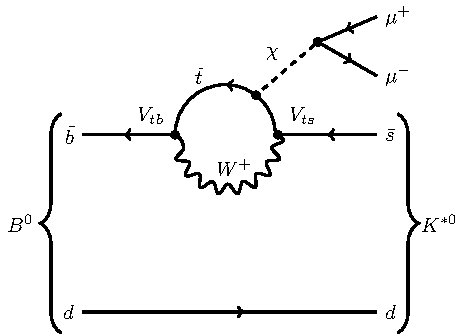
\includegraphics[scale=1]{feynman_inf}
  \caption{\small
    Feynman diagram showing the decay \btokstrdb, where the \db interacts by mixing with the
    Higgs or $Z$, which then decays into a dimuon pair.
  }
  \label{fig:feynman}
\end{center}
\end{figure}

The spin of the particle is not assumed either.
A similar analysis might search for a \db in \decay{\Bp}{\Kp\mumu}, where one might expect
additional sensitivity to scalar particles.
However, this is not the case.
Reference~\cite{Batell:2009jf} gives decay rates for decays of the type \decay{B}{K\db} to be:
\begin{align}
  \Gamma\big(\decay{B}{K\db}\big) &= \Gamma_0
  \frac{\lambda_{K}\big(m_{B}^2-m_{K}^2\big)^2}{m_{B}^6}
  \left[f_0\!\left(m_\db^2\right)\right]
  \\
  \Gamma\big(\decay{B}{\Kstar\db}\big) &= \Gamma_0
  \frac{\lambda_{\Kstar}^3}{m_{B}^6}
  \left[A_0\!\left(m_\db^2\right)\right]
  \\
  \intertext{where the phasespace factor is}
  \lambda_\kappa &= \left[
    \left( m_B^2 - m_\db^2 - m_\kappa^2 \right)^2
    -4m_\db^2m_\kappa^2
    \right]^\frac12,
    \label{eq:db:bx}
\end{align}
form factors are denoted as $f_0$ $A_0$, and $\Gamma_0$  is a constant.
Figure~\ref{fig:db:kx} shows that the phasespace factor is the dominant factor in the shape for all
the decays, and that searching for a particle, \db, in the decays \decay{\Bd}{\Kstarz\db} and
\decay{\Bp}{\Kp\db} is equally sensitive for $m_\db\lesssim2000\mev$.
%For example, Fig.~\ref{fig:th:kx} shows how the branching fraction of \decay{\Bd}{\Kstar\db} is
%expected to vary with the mass of the \db, in comparison to \decay{\Bd}{K\db}.


\begin{figure}
  \begin{center}
    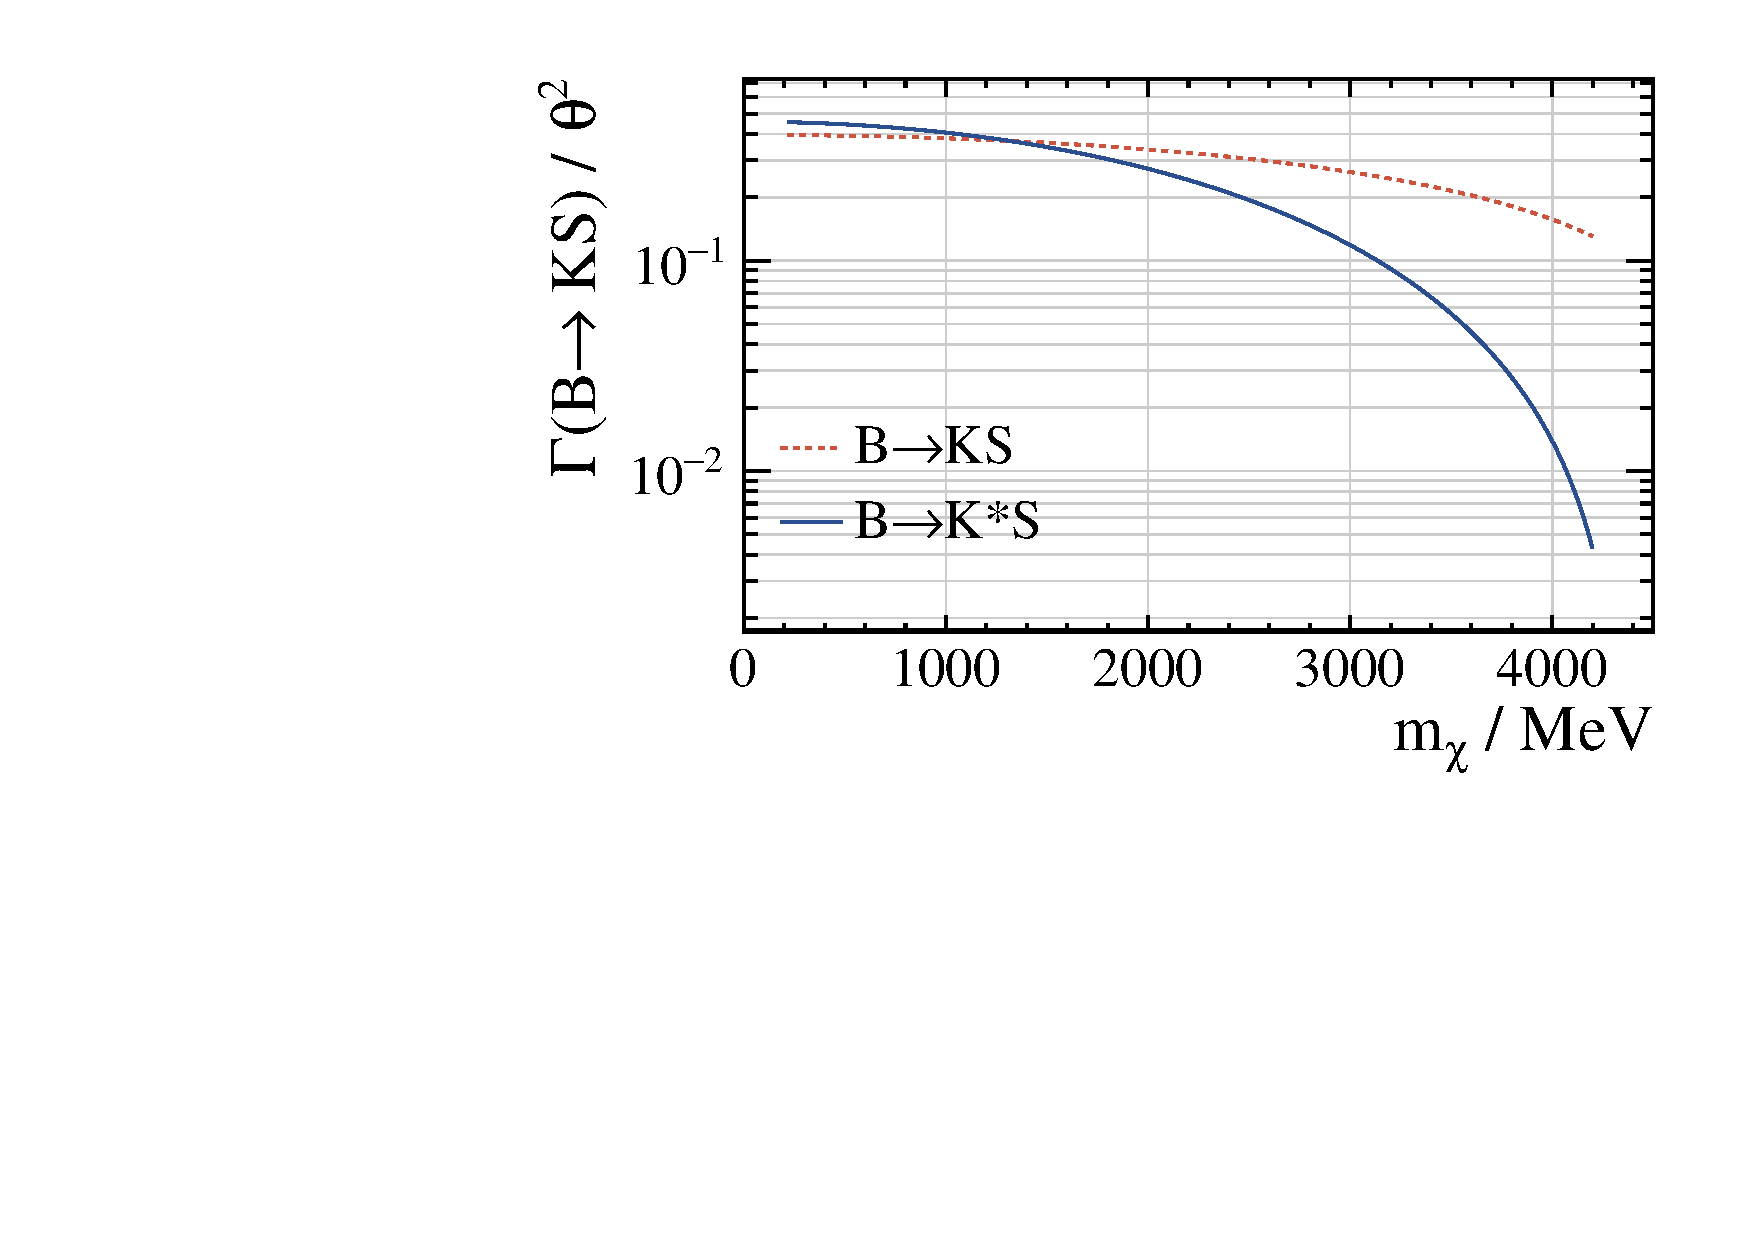
\includegraphics[width=0.48\textwidth]{bf_b2ks_root}
    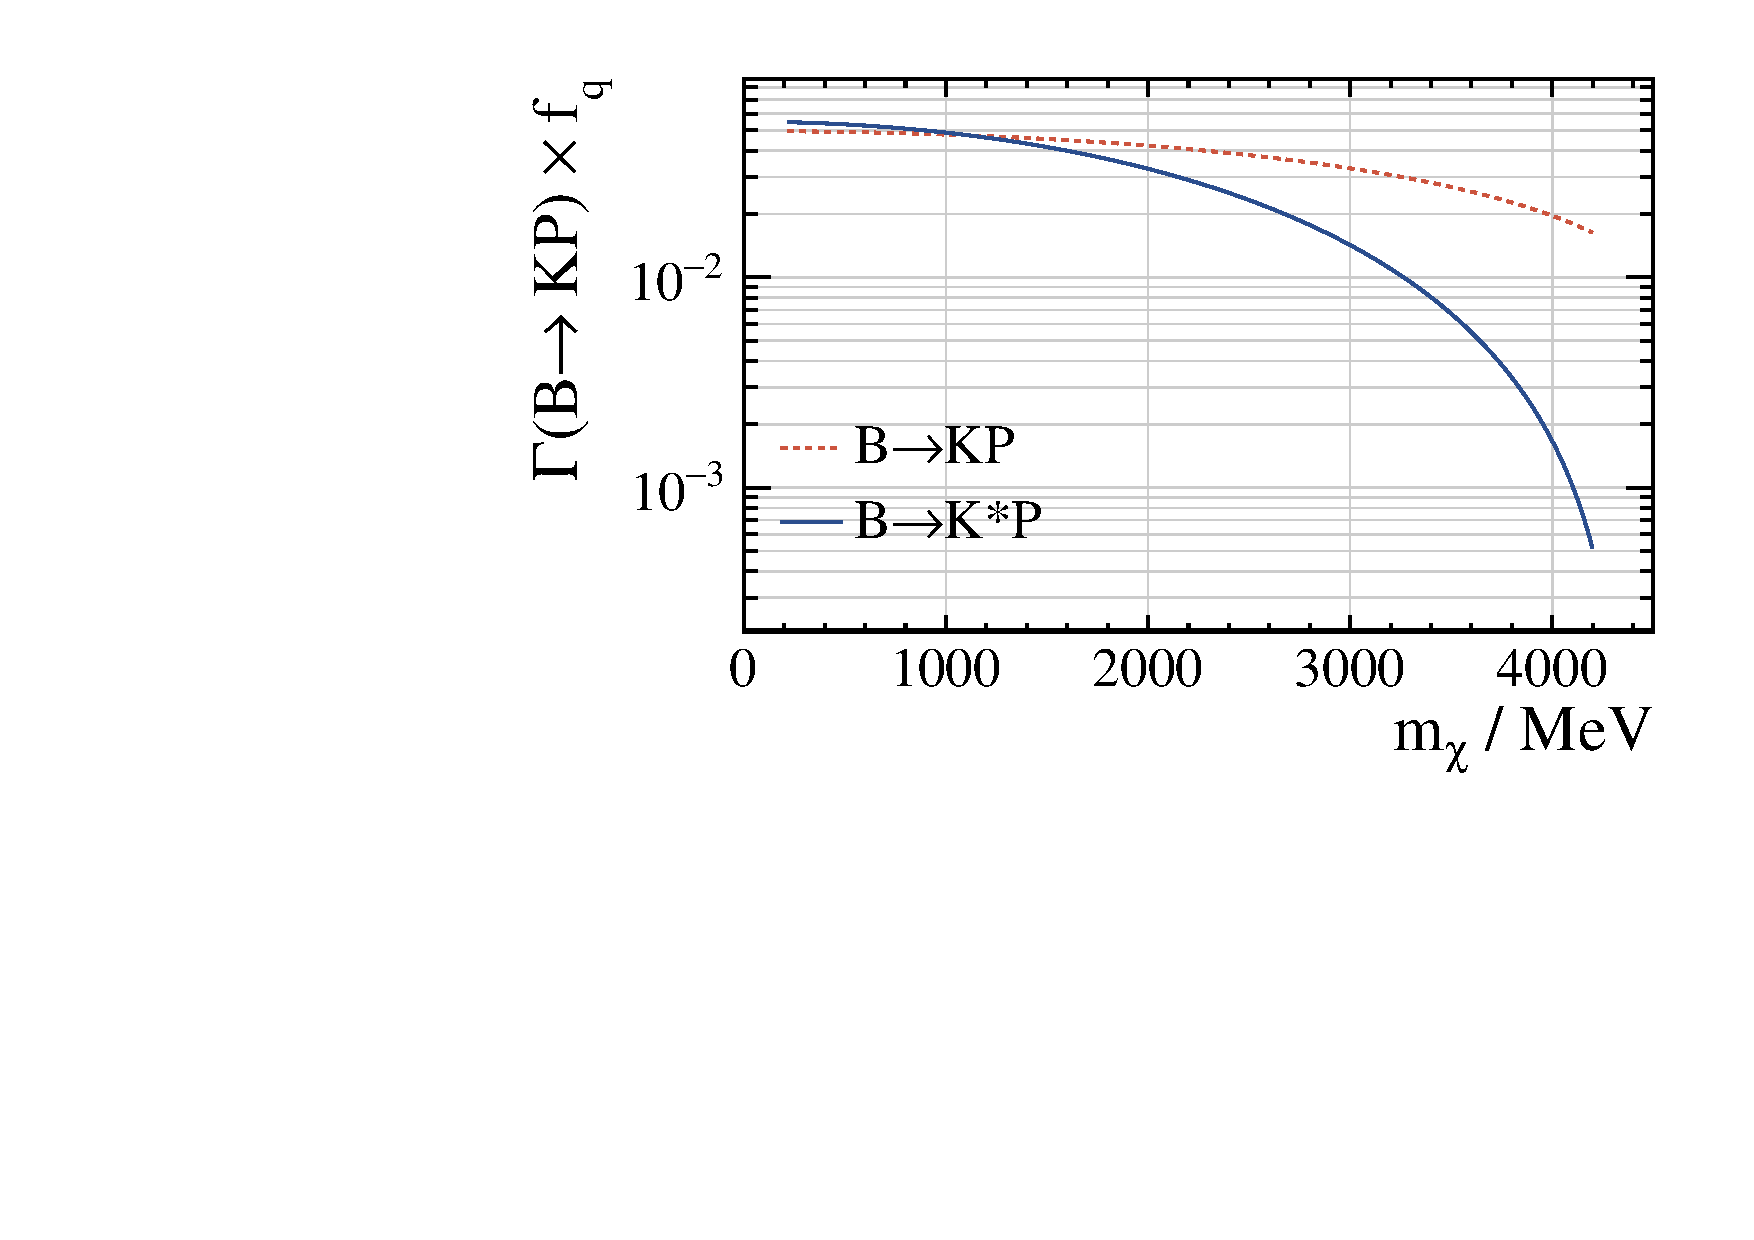
\includegraphics[width=0.48\textwidth]{bf_b2kv_root}
    \caption{\small
      Branching fraction predictions, from Eq.~\protect\ref{eq:db:bx},
      for decays of the form $\decay{B}{KX}$, where $X$ is either
      (left) a scalar (S) or
      (right) a vector (V).
      The parameters $\theta$ and $f_q$ are parameters of the model.
      %Note that for these plots $\mathrm{ln}\left(\Lambda_\mathrm{UV}/m_t\right)$ is set to one.
      The shapes of the curves are dominated by the available phasespace, and sensitivity is
      comparable for $m_\db\lesssim2000\mev$.
      %this is taken from Ref~\cite{Batell:2009jf}.
    }
    \label{fig:db:kx}
  \end{center}
\end{figure}


The following analysis is a fully frequentist search for a new particle \db, with an unknown mass
ans lifetime.
This is done in the two dimensions of mass and lifetime using the method described in
\Sec{sec:db:strategy}.


%The existence of dark matter in the universe is overwhelmingly supported by experimental evidence from galactic rotation curves, gravitational lensing, and acoustic modes in the CMB.
%As there are no viable dark matter candidate particles in the Standard Model (SM), new {\em dark} particles must exist.
%Dark matter provides strong evidence for a \emph{dark sector}, containing particles which only
%interact weakly with the spectrum of SM particles via mediating messenger particles, or
%\emph{Dark Bosons}.
%%Despite the countless successes of the Standard Model (SM), it is well known that it is an
%%incomplete picture of particle physics, failing, as it does, to explain a number of important
%%phenomena.
%%These range from theoretical problems of naturalness to experimental indications of Dark matter.
%%All of these point towards the existence of beyond SM physics, and the existence of an, as yet,
%%undiscovered particle.
%The following analysis note details the search for a hypothetical Dark Boson, \db, of
%unknown mass and lifetime.

%Many extensions of the SM predict the existence of a new light boson.
%As all interactions in the SM are gauged, it is reasonable to assume that the same can be said of
%interactions in the dark sector.
%If so, then they would contain new vector bosons such as so-called dark photons (referred to as
%$A^{\prime}$), dark $Z$ bosons (referred to as $Z_d$).
%%A particular model that would anticipate the observation of a light vector boson would one which
%%includes a dark $Z$ (or photon).
%%Such models are motivated by the existence of dark matter and also the $3.6\,\sigma$ deviation
%%exhibited between the theoretical and experimental measurements of the anomalous magnetic moment of
%%the muon, $a_\mu=\tfrac12(g_\mu-2)$~\cite{PDG2012}.
%A $Z_d$ that weakly couples to the visible sector with low mass
%($10\lesssim m_{Z_d}\lesssim500\mev$) would add corrections to the theoretical value of $a_\mu$
%bringing it in line with what is seen experimentally.
%Such models are outlined in Refs.~\cite{Davoudiasl:2012qa,Davoudiasl:2012ag,Lee:2014lga}.
%Other models might include such particles as Inflatons~\cite{Bezrukov:2009yw} and
%Axions~\cite{Peccei:2006as}.

%Many beyond SM regimes include a new boson which, as a result of electroweak symmetry breaking or a
%similar mechanism, couple to fermions proportionally to their mass.
%%In general, extensions to the SM often include bosons that couple to fermions proportionally to
%%their masses.
%%This occurs either due to mixing with the SM Higgs boson or due to the fact that the
%%new bosons arise via a symmetry breaking process similar to the Higgs mechanism.
%Therefore, processes that are mediated via loops that contain top quarks are excellent places to search for such particles.
%Figure~\ref{fig:feynman} shows a Feynman diagram of a potential process.
%
%\begin{figure}
  %\begin{center}
    %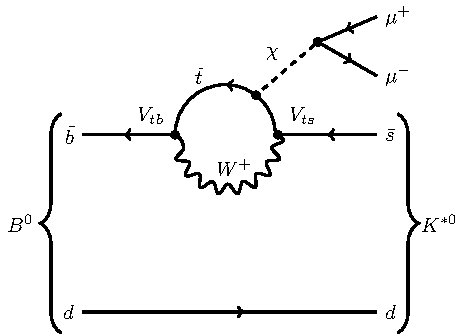
\includegraphics[scale=1]{feynman_inf}
  %\caption{\small
    %Feynman diagram showing the decay \btokstrdb, where the \db interacts by mixing with the
    %Higgs or $Z$, which then decays into a dimuon pair.
  %}
  %\label{fig:feynman}
%\end{center}
%\end{figure}

%%Many models which propose such a particle, but generally (for $m<m(B)$) they are dark
%%sector particles and only interact with the visible sector by mixing with the Higgs or $Z$ boson.
%%Some general theories predict particles known as:
%%\begin{itemize}
  %%\item Axions
  %%\item Any other generic beyond SM particle.
%%\end{itemize}
%
%In this analysis, a \db is searched for in the decay
%$\Bd\!\to K^*(892)^0\infl$, where $\Kstarz\!\to\Kp\pim$ and $\infl\!\to\mumu$
%(charge conjugation is assumed throughout this document, and unless explicitly
  %stated otherwise, $K^{*0}$ refers to the $K^*(892)^0$).
%The analysis is general in that no mass, lifetime or spin is assumed for \db.
%%This search is sensitive to both vector and scalar particles.
%For example, Fig.~\ref{fig:th:kx} shows how the branching fraction of \decay{\Bd}{\Kstar\db} is
%expected to vary with the
%mass of the \db, in comparison to \decay{\Bd}{K\db}.
%This is the case for a scalar or vector \db.
%
%In the dimuon mass region below the $J/\psi$ mass, both the $K$ and \Kstar decay modes are roughly
%equally sensitive to vector and scalar particles.
%%Appendix~\ref{app:np} provides more details on beyond the SM theories which include a particle
%%that this search could be sensitive to.
%
%\begin{figure}
  %\begin{center}
    %\subfloat[\label{fig:th:ks}]{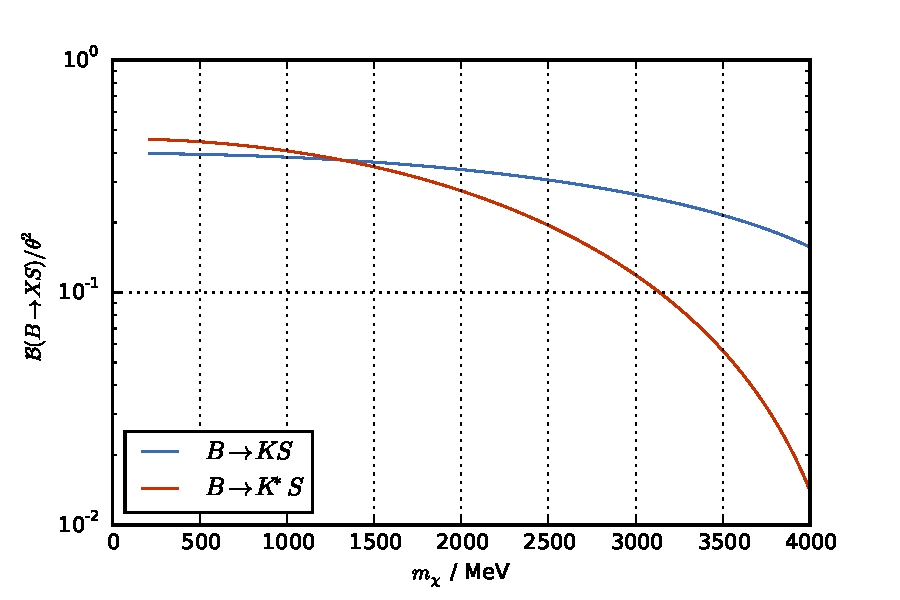
\includegraphics[width=0.48\textwidth]{bf_b2ks}}
    %\subfloat[\label{fig:th:kv}]{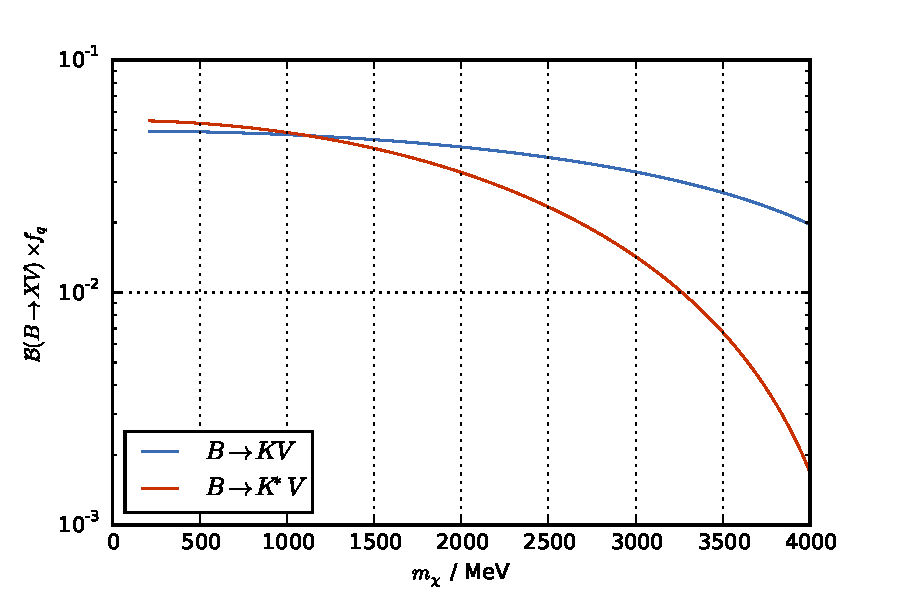
\includegraphics[width=0.48\textwidth]{bf_b2kv}}
    %\caption{\small
      %Branching fraction distributions %from Eq.~\protect\ref{eq:th:bx}
      %for $\decay{B}{KX}$ where $X$ is either
      %\protect\subref{fig:th:ks} a scalar (S) or
      %\protect\subref{fig:th:kv} a vector (V).  Note that for these plots
      %$\mathrm{ln}\left(\Lambda_\mathrm{UV}/m_t\right)$ is set to one.
      %The shapes of the curves are dominated by the available phasespace, this is taken
      %from Ref~\cite{Batell:2009jf}.
    %}
    %\label{fig:th:kx}
  %\end{center}
%\end{figure}
%
%
%
%
%\section{New physics scenarios}
%\label{app:np}
%
%\subsection{New scalar particles}
%In this search we are looking for $\decay{\Bd}{K^*(892)^0\db}$, and since the \Bd is a
%psuedoscalar, and
%the $K^*(892)^0$ is a vector; nai\"{i}vely one might expect that the \db must also be a vector.
%However, this is not the case.
%The equations given in Ref.~\cite{Batell:2009jf}:
%\begin{align}
  %\BF(\decay{B}{KS})
  %&=4\e{-7}\times\left(\frac{\theta}{10^{-3}}\right)^2
  %\mathcal{F}_K^2(m_S)\lambda^\frac12_{KS} \nonumber\\
  %\BF(\decay{B}{K^*S})
  %&=5\e{-7}\times\left(\frac{\theta}{10^{-3}}\right)^2
  %\mathcal{F}_K^{*2}(m_S)\lambda^\frac32_{K^*S} \nonumber\\
  %\BF(\decay{B}{KV})
  %&=5\e{-6}\times
  %\left[ \frac{100\tev}{f_q}\mathrm{ln}\left(\frac{\Lambda_\mathrm{UV}}{m_t}\right) \right]^2
  %\mathcal{F}_K^2(m_V)\lambda^\frac12_{KV} \nonumber\\
  %\BF(\decay{B}{K^*V})
  %&=6\e{-6}\times
  %\left[ \frac{100\tev}{f_q}\mathrm{ln}\left(\frac{\Lambda_\mathrm{UV}}{m_t}\right) \right]^2
  %\mathcal{F}_K^2(m_V)\lambda^\frac32_{K^*V} \nonumber
  %\label{eq:th:bx}
%\end{align}
%where
%\begin{equation}
  %\lambda_{ij} = \frac{1}{m_B^4}
  %\left(m_b^2 - \left(m_i+m_j\right)^2\right)
  %\left(m_b^2 - \left(m_i-m_j\right)^2\right)
%\end{equation}
%is the phasespace term and $\mathcal{F}$ are form factors.
%Branching fraction distributions for the scalar and vector dark bosons are shown in
%\Fig{fig:th:kx}, these show that the branching fraction for the $K^*$ mode is greater for
%$m_\db\lesssim1250\mev$ compared to the $K$ mode.
%
%
%\subsection{Axions}
%A gauge invariant term that can be added to $\Lag{QCD}$ is
%\begin{equation}
  %\Lag{QCD}^\theta = \theta\frac{g^2}{32\pi^2}
  %F_{\mu\nu}^\alpha\widetilde F^{\mu\nu}_\alpha,
%\end{equation}
%where $\theta$ and $g$ are constants, and $\alpha$ indicates a sum over colours.
%The operator $F_{\mu\nu}$ is the gluon field strength tensor, and
%\begin{equation}
  %\widetilde F^{\mu\nu}_\alpha = \frac12\varepsilon_{\mu\nu\rho\sigma}F^{\rho\sigma}_\alpha.
%\end{equation}
%An interaction such $\Lag{QCD}^\theta$ would conserve charge symmetry, but violate parity and time
%conjugation~\cite{Peccei:2006as}.
%Such symmetry violations are in contradiction with the observed properties of the strong
%force.
%Bounds placed on the value of the neutron dipole moment, $|d_n| <2.9\e{-26}\,\mathrm{ecm}$
%(at 90\% CL)~\cite{Baker:2006ts} requires $\theta$ to be very small,
%$\theta<10^{-19}$~\cite{Crewther:PQref9}, when \emph{a priori} it could be in the range
%$0<\theta<2\pi$.
%This occurrence of fine tuning is referred to as the \emph{strong CP problem}.
%A solution to this problem is to introduce an additional chiral symmetry, such that $\theta$
%becomes a field, the quanta of which are called axions.
%%A solution of the strong CP problem is to introduce a chiral $U(1)$ symmetry which is spontaneously
%%broken and effectively replaces the CP violating angle $\theta$ with a CP conserving field.
%
%
%
%\subsection{Inflatons}
%Cosmological inflation in the early universe (very early, $t=10^{-35}$ to $10^{-34}$\,s can be put
%down to the existence of a scalar field that weakly couples to SM particles via some mixing with the
%Higgs sector.
%Before expansion, the inflation field was at a higher energy state.
%Quantum fluctuations caused a phase transition where the inflaton field released its potential
%energy as matter radiation as it settled to its lowest energy state,
%This action generated a repulsive force that drove the portion of the universe that is observable
%today to accelerate in expansion.
%Many of such theories predict the mass of the scalar to be massive, potentially beyond the reach of
%the \lhc.
%However, there is hope, Ref.~\cite{Bezrukov:2009yw} outlines possibilities for the inflaton to be in
%the range $270 < m(\infl) < 10000$\mev.
%
%This model has a Lagrangian which looks like:
%\begin{align}
  %\Lag{tot} &= \Lag{SM} + \Lag{\db} \\
  %\Lag{\db} &= \frac12\partial_\mu\infl\partial^\mu\infl
  %+\frac12m(\infl)^2\infl^2
  %-\frac\beta4\infl^4
  %-\lambda\left(H^\dagger H-\frac\alpha\lambda\infl^2\right)^2.
  %\label{eq:laginf}
%\end{align}
%Where the term $\Lag{SM}$ is the SM Lagrangian without the Higgs potential, which gets
%modified to that shown in Eq.~\ref{eq:laginf}
%


